\documentclass{article}
% 基础配置：中文支持+核心数学包
\usepackage[fontset=windows,UTF8]{ctex}
\usepackage{amsmath,amssymb,amsfonts,mathtools}
% 基础排版包
\usepackage{geometry,enumitem,graphicx,amsthm,booktabs,hyperref,multicol}
% 辅助包
\usepackage{ragged2e}
\usepackage{setspace}
\usepackage{titlesec}
\usepackage{titletoc}
\usepackage{fancyhdr}
\usepackage{xcolor}
\usepackage{lastpage} % 确保正确加载lastpage包
% 新增：嵌入视频需要的包
\usepackage{media9}

% 定义缺失的darkblue颜色
\definecolor{darkblue}{RGB}{0,0,128}

% 页面设置
\geometry{a4paper, margin=1in}
\setstretch{1.2}
\setlength{\parskip}{0.6em}
\setlength{\parindent}{0pt}
\sloppy % 解决Underfull \hbox警告

% 自定义命令
\newcommand{\Cov}{\mathrm{Cov}}
\newcommand{\E}{\mathrm{E}}
\newcommand{\D}{\mathrm{Var}}
\newcommand{\Prob}{\mathrm{P}}
\newcommand{\dif}{\mathop{}\!\mathrm{d}}
\newcommand{\e}{\mathrm{e}}
\newcommand{\indep}{\perp \!\!\! \perp}
\newcommand{\samplemean}[1]{\overline{#1}}
\newcommand{\samplevar}[1]{S_{#1}^2}
\newcommand{\symnote}[1]{\par\noindent\textbf{符号说明：}#1\par}
\newcommand{\maxrv}[2]{\max\left\{#1,#2\right\}}
\newcommand{\minrv}[2]{\min\left\{#1,#2\right\}}
\newcommand{\ualpha}{u_{\alpha/2}}
\newcommand{\talpha}[1]{t_{\alpha/2}(#1)}
\newcommand{\xalpha}[1]{\chi^2_{\alpha/2}(#1)}
\newcommand{\xalphaone}[1]{\chi^2_{1-\alpha/2}(#1)}

% 定理环境
\newtheoremstyle{mytheorem}{10pt}{10pt}{\normalfont}{0pt}{\bfseries}{：}{0.5em}{}
\theoremstyle{mytheorem}
\newtheorem{theorem}{定理}[section]
\newtheorem{definition}{定义}[section]
\newtheorem{property}{性质}[section]
\newtheorem{corollary}{推论}[section]
\newtheorem{example}{例}[section]

% 超链接（已整合作者信息）
\hypersetup{
    colorlinks=true,
    linkcolor=blue,
    urlcolor=cyan,
    citecolor=red,
    pdftitle={概率论与数理统计核心公式整理},
    pdfauthor={Duckweed-yhb},
    pdfsubject={概率论与数理统计},
    pdfpagemode=UseOutlines,
    hidelinks,
    unicode=true % 解决中文链接问题
}

% 列表样式
\setlist[enumerate]{
    label=(\roman*),
    leftmargin=2em,
    itemsep=0.3em,
    parsep=0.1em
}
\setlist[itemize]{
    leftmargin=2em,
    itemsep=0.3em,
    parsep=0.1em
}
\setlist[enumerate,1]{label=\arabic*., leftmargin=2em, itemsep=0.8em, parsep=0.2em}

% 标题格式
\titleformat{\section}
  {\Large\bfseries\centering\color{darkblue}}
  {\thesection}
  {0.8em}
  {}
\titleformat{\subsection}
  {\large\bfseries\color{darkblue}}
  {\thesubsection}
  {0.8em}
  {}

% 目录
\titlecontents{section}
  [0pt]
  {\bfseries}
  {\thecontentslabel\quad}
  {}
  {\ \titlerule*[0.5pc]{.}\contentspage}
\titlecontents{subsection}
  [1.5em]
  {}
  {\thecontentslabel\quad}
  {}
  {\ \titlerule*[0.5pc]{.}\contentspage}

% 页眉页脚
\pagestyle{fancy}
\fancyhf{}
\renewcommand{\headrulewidth}{0.4pt}
\renewcommand{\footrulewidth}{0.2pt}
\fancyhead[L]{\footnotesize 概率论与数理统计}
\fancyhead[R]{\footnotesize \leftmark}
\fancyfoot[C]{\footnotesize 第 \thepage 页 / 共 \pageref{LastPage} 页}
\fancypagestyle{plain}{
    \fancyhf{}
    \renewcommand{\headrulewidth}{0pt}
    \renewcommand{\footrulewidth}{0.2pt}
    \fancyfoot[C]{\footnotesize 第 \thepage 页 / 共 \pageref{LastPage} 页}
}

% 封面命令（核心修改：视频长宽比适配16:9，优化参数稳定性）
\newcommand{\makeCover}{
    \begin{titlepage}
        \centering
        % 减少顶部空白，让文字上移
        \vspace*{1.5cm}
        {\Huge \bfseries 概率论与数理统计}\\[12pt]
        {\Huge \bfseries 核心公式整理}\\[24pt]
        {\Large \itshape —— 完整版复习讲义 ——}\\[1cm]
        
        % 作者信息区块
        {\Large \textbf{整理者：}Duckweed-yhb}\\[8pt]
        {\large \textbf{个人博客：}\url{https://duckweed-yhb.github.io/}}\\[8pt]
        {\large \textbf{GitHub：}\url{https://github.com/Duckweed-yhb}}\\[8pt]
        {\large \textbf{联系邮箱：}\href{mailto:3071974740@qq.com}{3071974740@qq.com}}\\[8pt]
        {\Large 日期：\today}\\[1cm]
        
        % 嵌入MP4视频（核心修改：长宽比适配16:9）
        \textbf{相关视频：}\\[6pt]
        \includemedia[
            width=0.8\textwidth,
            height=0.45\textwidth, % 16:9比例：0.8 * 9/16 = 0.45
            activate=pageopen,      % 页面打开时激活视频
            addresource={guidao.mp4}, % 视频文件名
            flashvars={
                source=guidao.mp4    % 对应视频文件名
                &autoPlay=true       % 自动播放
                &loop=true           % 循环播放
                &controlBarVisible=true % 显示控制栏
                &volume=100          % 音量100%
                &playButtonVisible=false % 隐藏播放按钮
                &scaleMode=letterbox % 保持视频比例，避免拉伸
            }
        ]{\fbox{\parbox{0.75\textwidth}{\centering 视频自动播放中...}}}{VPlayer.swf}
        
        \vfill
    \end{titlepage}
}

\begin{document}

% 封面
\makeCover
\clearpage

% 目录页
\pagenumbering{Roman}
\tableofcontents
\clearpage
\pagenumbering{arabic}

\section{随机事件与概率}
\subsection{条件概率与独立性}
\begin{theorem}[泊松逼近定理]
如果 $n \to \infty$，$p \to 0$ 使得 $np = \lambda$ 保持为正常数，则
$$
\mathrm{C}_{n}^{k}p^{k}(1 - p)^{n - k} \to \frac{\lambda^{k}}{k!}\e^{-\lambda}
$$
对 $k = 0,1,2,\cdots$ 一致地成立。
\symnote{$\mathrm{C}_n^k$：组合数；$p$：单次试验成功概率；$\lambda$：泊松分布参数；$\e$：自然常数。}
\end{theorem}

\section{随机变量及其分布}
\subsection{七种常用分布表}
\noindent 注：将图片命名为“七种常用分布表.jpg”放在同目录下 \\
\IfFileExists{七种常用分布表.jpg}{
  \centering
  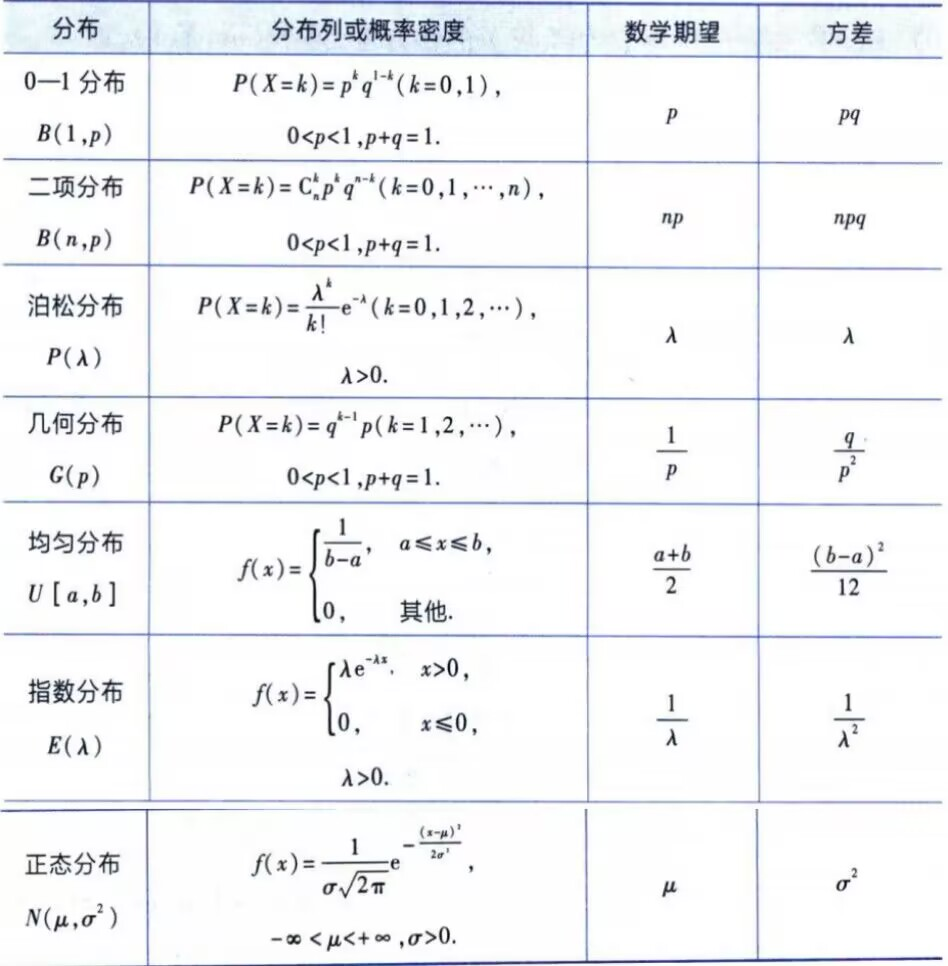
\includegraphics[width=0.9\textwidth, keepaspectratio]{七种常用分布表.jpg}
  \par
}{
  \textbf{提示：未找到“七种常用分布表.jpg”，请检查路径！}
}

\subsection{分布函数与概率密度}
\begin{definition}[分布函数]
设 $X$ 为随机变量，称 $F(x) = \Prob(X \leq x)$ 为 $X$ 的分布函数（$x$ 为任意实数）。
\symnote{$F(x)$：分布函数；$\Prob(\cdot)$：概率运算符。}
\end{definition}

\begin{definition}[概率密度]
设 $F(x)$ 是 $X$ 的分布函数，若存在非负函数 $f(x)$ 使得
$$
F(x)=\int_{-\infty}^{x} f(t) \dif t
$$
则称 $X$ 为连续型随机变量，$f(x)$ 为其概率密度。
\symnote{$f(x)$：概率密度；$\dif t$：微分符号。}
\end{definition}

\subsection{正态分布}
\begin{definition}[标准正态分布]
正态分布 $N(\mu,\sigma^2)$ 中 $\mu=0, \sigma=1$ 时为标准正态分布 $N(0,1)$，其概率密度与分布函数：
$$
\varphi(x)=\frac{1}{\sqrt{2\pi}} \e^{-\frac{x^2}{2}} \quad (-\infty < x < +\infty)
$$
$$
\Phi(x)=\frac{1}{\sqrt{2\pi}} \int_{-\infty}^{x} \e^{-\frac{t^2}{2}} \dif t \quad (-\infty < x < +\infty)
$$
\symnote{$\varphi(x)$：标准正态PDF；$\Phi(x)$：标准正态CDF；$\pi$：圆周率。}
\end{definition}

\begin{property}[标准正态分布的对称性]
$\varphi(x)$ 是偶函数，满足：
$$
\varphi(-x)=\varphi(x), \quad \Phi(-x)=1-\Phi(x)
$$
\end{property}

\begin{property}[一般正态分布的标准化]
若 $X \sim N(\mu,\sigma^2)$，则 $F(x)=\Phi\left( \frac{x-\mu}{\sigma} \right)$，区间概率：
$$
\Prob(x_1 < X \leq x_2)=\Phi\left( \frac{x_2-\mu}{\sigma} \right)-\Phi\left( \frac{x_1-\mu}{\sigma} \right) \quad (x_1 < x_2)
$$
\symnote{$\mu$：均值；$\sigma$：标准差；$F(x)$：一般正态CDF。}
\end{property}

\begin{theorem}[随机变量函数的概率密度]
设 $X$ 为连续型随机变量，概率密度 $f(x)$，$Y = g(X)$。若 $g(x)$ 逐段严格单调，反函数 $h_i(y)$ 且导数连续，则
$$
f_Y(y) = \sum_{i} f\bigl(h_i(y)\bigr)\left|h_i'(y)\right|
$$
（无意义的 $y$ 处，$f_Y(y)=0$）
\symnote{$f_Y(y)$：$Y$的概率密度；$h_i'(y)$：反函数导数；$|\cdot|$：绝对值。}
\end{theorem}

\section{多维随机变量及其分布}
\subsection{联合分布函数}
\begin{definition}[二维联合分布函数]
设 $(X,Y)$ 为二维随机变量，$x,y$ 为任意实数，称
$$
F(x,y) = \Prob(X \leq x, Y \leq y)
$$
为 $(X,Y)$ 的联合分布函数。
\symnote{$F(x,y)$：二维联合分布函数。}
\end{definition}

\begin{property}[联合分布函数的基本性质]
\begin{enumerate}
    \item 有界性：$0 \le F(x,y) \le 1$；
    \item 单调不减性：$x_1 < x_2 \implies F(x_1,y) \le F(x_2,y)$，$y_1 < y_2 \implies F(x,y_1) \le F(x,y_2)$；
    \item 极限性质：$F(-\infty,y)=F(x,-\infty)=F(-\infty,-\infty)=0, F(+\infty,+\infty)=1$；
    \item 右连续性：$F(x,y) = F(x^+,y) = F(x,y^+)$；
    \item 非负性：$x_1 \le x_2, y_1 \le y_2$ 时，$F(x_2,y_2) - F(x_2,y_1) - F(x_1,y_2) + F(x_1,y_1) \ge 0$。
\end{enumerate}
\end{property}

\subsection{边缘分布}
\begin{definition}[边缘分布函数]
设 $(X,Y)$ 的联合分布函数为 $F(x,y)$，则：
\begin{itemize}
    \item $X$ 的边缘分布函数：$F_X(x) = \lim_{y \to +\infty} F(x,y)$；
    \item $Y$ 的边缘分布函数：$F_Y(y) = \lim_{x \to +\infty} F(x,y)$。
\end{itemize}
\symnote{$F_X(x)$：$X$边缘CDF；$F_Y(y)$：$Y$边缘CDF；$\lim$：极限运算符。}
\end{definition}

\begin{definition}[二维离散型随机变量的联合分布列]
设 $(X,Y)$ 所有可能取值为 $(x_i, y_j)$（$i,j=1,2,\dots$），记
$$
p_{ij} = \Prob(X = x_i, Y = y_j)
$$
为联合分布列，满足：非负性 $p_{ij} \ge 0$；规范性 $\sum_i \sum_j p_{ij} = 1$；边缘分布列 $p_{i.} = \sum_j p_{ij}, p_{.j} = \sum_i p_{ij}$。
\symnote{$p_{ij}$：联合概率；$p_{i.}/p_{.j}$：边缘概率；$\sum$：求和运算符。}
\end{definition}

\begin{definition}[二维连续型随机变量的联合概率密度]
设 $(X,Y)$ 的分布函数为 $F(x,y)$，若存在非负函数 $f(x,y)$ 使得
$$
F(x,y) = \int_{-\infty}^x \int_{-\infty}^y f(u,v)\dif u\dif v
$$
则称 $f(x,y)$ 为联合概率密度，边缘概率密度：
$$
f_X(x) = \int_{-\infty}^{+\infty} f(x,y)\dif y, \quad f_Y(y) = \int_{-\infty}^{+\infty} f(x,y)\dif x
$$
\symnote{$f(x,y)$：二维联合PDF；$f_X(x)/f_Y(y)$：边缘PDF。}
\end{definition}

\subsection{独立性}
\begin{definition}[随机变量的独立性]
若对任意实数 $x,y$，有 $F(x,y) = F_X(x) F_Y(y)$，则称 $X$ 与 $Y$ 相互独立（记为 $X \indep Y$）。
\symnote{$\indep$：独立符号。}
\end{definition}

\begin{property}[独立性的充要条件]
\begin{itemize}
    \item 连续型：$f(x,y) = f_X(x) f_Y(y)$；
    \item 离散型：$p_{ij} = p_{i.} p_{.j} \ (\forall i,j)$。
\end{itemize}
\end{property}

\subsection{二维随机变量函数的分布}
\begin{property}[和的分布（卷积公式）]
若 $X \indep Y$，概率密度分别为 $f_X(x), f_Y(y)$，则 $Z = X + Y$ 的概率密度：
$$
f_Z(z) = \int_{-\infty}^{+\infty} f_X(x) f_Y(z - x) \dif x = \int_{-\infty}^{+\infty} f_X(z - y) f_Y(y) \dif y
$$
\symnote{$f_Z(z)$：$Z=X+Y$的概率密度。}
\end{property}

\begin{property}[$\max\{X,Y\}$ 与 $\min\{X,Y\}$ 分布（独立情形）]
设 $X$ 与 $Y$ 相互独立，边缘分布函数分别为 $F_X(x)$ 和 $F_Y(y)$：
\begin{enumerate}[label=\arabic*.]
    \item 最大值 $M = \maxrv{X}{Y}$
    分布函数：
    $$
    F_M(m) = F_X(m) \cdot F_Y(m)
    $$
    连续型概率密度：
    $$
    f_M(m) = f_X(m) \cdot F_Y(m) + F_X(m) \cdot f_Y(m)
    $$

    \item 最小值 $N = \minrv{X}{Y}$
    分布函数：
    $$
    F_N(n) = 1 - [1 - F_X(n)] \cdot [1 - F_Y(n)]
    $$
    连续型概率密度：
    $$
    f_N(n) = f_X(n) \cdot [1 - F_Y(n)] + [1 - F_X(n)] \cdot f_Y(n)
    $$
\end{enumerate}
\symnote{$\maxrv{X}{Y}$：最大值；$\minrv{X}{Y}$：最小值；$f_M(m)/f_N(n)$：对应PDF。}
\end{property}

\begin{example}[max/min分布计算示例]
设$X,Y$独立同分布于$U(0,1)$，则：
\begin{itemize}
    \item $F_X(x)=F_Y(x)=\begin{cases}0, & x<0 \\ x, & 0\leq x\leq1 \\ 1, & x>1\end{cases}$

    \item $M=\maxrv{X}{Y}$的分布函数（CDF）：
    $$
    F_M(m)=\begin{cases}0, & m<0 \\ m^2, & 0\leq m\leq1 \\ 1, & m>1\end{cases}
    $$

    \item $N=\minrv{X}{Y}$的分布函数（CDF）：
    $$
    F_N(n)=\begin{cases}0, & n<0 \\ 1-(1-n)^2, & 0\leq n\leq1 \\ 1, & n>1\end{cases}
    $$
\end{itemize}
\end{example}

\begin{definition}[瑞利分布]
设 $X$ 服从参数为 $\sigma > 0$ 的瑞利分布，则：
\begin{itemize}
    \item PDF：$f(x) = \begin{cases}\dfrac{x}{\sigma^2} \e^{-\dfrac{x^2}{2\sigma^2}} & x \ge 0, \\ 0 & x < 0.\end{cases}$
    \item CDF：$F(x) = \begin{cases}1 - \e^{-\dfrac{x^2}{2\sigma^2}} & x \ge 0, \\ 0 & x < 0.\end{cases}$
\end{itemize}
\symnote{$\sigma$：瑞利分布参数；PDF：概率密度；CDF：分布函数。}
\end{definition}

\section{随机变量的数字特征与极限定理}
\subsection{数学期望}
\begin{definition}[数学期望]
\begin{itemize}
    \item 离散型：$\E(X) = \sum_{i=1}^{\infty} x_i p_i$（条件 $\sum_{i=1}^{\infty} |x_i| p_i < +\infty$）；
    \item 连续型：$\E(X) = \int_{-\infty}^{+\infty} x f(x) \dif x$（条件 $\int_{-\infty}^{+\infty} |x| f(x) \dif x < +\infty$）。
\end{itemize}
\symnote{$\E(X)$：数学期望；$|x|$：绝对值。}
\end{definition}

\begin{property}[数学期望的性质]
设 $C$ 为常数，$X,X_1,\dots,X_n$ 为随机变量：
\begin{enumerate}
    \item $\E(C) = C$；
    \item $\E(CX) = C\E(X)$；
    \item 线性性：$\E\left(\sum_{i=1}^n X_i\right) = \sum_{i=1}^n \E(X_i)$（无需独立）；
    \item 独立乘积：若 $X_1,\dots,X_n$ 独立，则 $\E\left(\prod_{i=1}^n X_i\right) = \prod_{i=1}^n \E(X_i)$。
\end{enumerate}
\symnote{$\prod$：乘积运算符。}
\end{property}

\subsection{方差}
\begin{definition}[方差]
$$
\D(X) = \E\left[X-\E(X)\right]^2 = \E(X^2) - \left[\E(X)\right]^2
$$
标准差：$\sigma_X = \sqrt{\D(X)}$。
\symnote{$\D(X)$：方差；$\sigma_X$：标准差；$\sqrt{\cdot}$：平方根。}
\end{definition}

\begin{property}[方差的性质]
设 $C$ 为常数，$X,Y,X_1,\dots,X_n$ 为随机变量：
\begin{enumerate}
    \item $\D(C) = 0$；
    \item $\D(CX) = C^2 \D(X)$；
    \item 独立和：若 $X_1,\dots,X_n$ 独立，则 $\D\left(\sum_{i=1}^n X_i\right) = \sum_{i=1}^n \D(X_i)$；
    \item $\D(XY) = \D(X)\D(Y) + \D(X)\left[\E(Y)\right]^2 + \D(Y)\left[\E(X)\right]^2$（$X \indep Y$）；
    \item $\D(X) = 0 \iff \Prob(X = \E(X)) = 1$。
\end{enumerate}
\symnote{$\iff$：充要条件。}
\end{property}

\subsection{协方差与相关系数}
\begin{definition}[协方差]
$$
\Cov(X,Y) = \E\left\{[X-\E(X)][Y-E(Y)]\right\} = \E(XY) - \E(X)\E(Y)
$$
\symnote{$\Cov(X,Y)$：协方差。}
\end{definition}

\begin{property}[协方差的性质]
\begin{enumerate}
    \item 对称性：$\Cov(X, Y) = \Cov(Y, X)$；
    \item 数乘：$\Cov(aX, bY) = ab\Cov(X, Y)$；
    \item 可加性：$\Cov(X_1 + X_2, Y) = \Cov(X_1, Y) + \Cov(X_2, Y)$。
\end{enumerate}
\end{property}

\begin{definition}[相关系数]
$$
\rho_{XY} = \frac{\Cov(X,Y)}{\sqrt{\D(X)}\sqrt{\D(Y)}}
$$
若 $\rho_{XY}=0$，称 $X$ 与 $Y$ 不相关。
\symnote{$\rho_{XY}$：相关系数；不相关：线性相关性为0。}
\end{definition}

\begin{property}[相关系数的性质]
\begin{enumerate}
    \item 有界性：$|\rho_{XY}| \le 1$；
    \item $|\rho_{XY}| = 1 \iff \Prob(Y = a + bX) = 1$（线性相关）；
    \item 不相关等价：$\Cov(X,Y)=0 \iff \D(X+Y)=\D(X)+\D(Y) \iff \E(XY)=\E(X)\E(Y)$。
\end{enumerate}
\end{property}

\subsection{矩}
\begin{definition}[矩的定义]
\begin{enumerate}
    \item 单个随机变量的矩：
    \begin{itemize}
        \item $k$ 阶原点矩：$\alpha_k = \E(X^k)$；
        \item $k$ 阶中心矩：$\beta_k = \E\left\{[X-\E(X)]^k\right\}$；
    \end{itemize}
    \item 两个随机变量的混合矩：
    \begin{itemize}
        \item $k+l$ 阶混合原点矩：$\alpha_{k,l} = \E(X^k Y^l)$；
        \item $k+l$ 阶混合中心矩：$\beta_{k,l} = \E\left\{[X-\E(X)]^k [Y-\E(Y)]^l\right\}$。
    \end{itemize}
\end{enumerate}
\symnote{$k,l$：矩的阶数（正整数）。}
\end{definition}

\subsection{大数定律与中心极限定理}
\begin{theorem}[切比雪夫不等式]
对任意 $\varepsilon > 0$，有
$$
\Prob\left[|X-\E(X)| \ge \varepsilon\right] \le \frac{\D(X)}{\varepsilon^2}
$$
\symnote{$\varepsilon$：误差界；$\varepsilon^2$：平方。}
\end{theorem}

\begin{theorem}[伯努利大数定律]
设 $Y_n$ 为 $n$ 重伯努利试验成功次数，成功概率 $p$，则
$$
\lim_{n \to \infty} \Prob\left(\left|\frac{Y_n}{n} - p\right| \ge \varepsilon\right) = 0
$$
\symnote{$Y_n$：成功次数；$n$：试验次数；$\lim$：极限。}
\end{theorem}

\begin{theorem}[辛钦大数定律]
若 $X_1,X_2,\dots$ 独立同分布，$\E(X_i)=\mu$，则
$$
\lim_{n \to \infty} \Prob\left(\left|\frac{1}{n}\sum_{i=1}^n X_i - \mu\right| \ge \varepsilon\right) = 0
$$
\symnote{$\mu$：共同均值；$\frac{1}{n}\sum_{i=1}^n X_i$：样本均值。}
\end{theorem}

\begin{theorem}[独立同分布中心极限定理]
若 $X_1,X_2,\dots$ 独立同分布，$\E(X_i)=\mu, \D(X_i)=\sigma^2>0$，则
$$
\lim_{n \to \infty} \Prob\left( \frac{1}{\sqrt{n}\sigma} \left( \sum_{i=1}^n X_i - n\mu \right) \le x \right) = \Phi(x)
$$
\end{theorem}

\begin{theorem}[棣莫弗-拉普拉斯定理]
设 $Y_n \sim B(n,p)$，$q=1-p$，则
$$
\lim_{n \to \infty} \Prob\left( \frac{Y_n - np}{\sqrt{npq}} \le x \right) = \Phi(x)
$$
\symnote{$B(n,p)$：二项分布；$q$：失败概率；$\sqrt{npq}$：二项分布标准差。}
\end{theorem}

\section{数理统计的基本概念}
\subsection{常用抽样分布}
\begin{definition}[$\chi^2$ 分布]
若 $X_1,\dots,X_n \indep N(0,1)$，则 $Y = \sum_{i=1}^n X_i^2 \sim \chi^2(n)$（自由度 $n$），满足：
\begin{enumerate}
    \item 可加性：$X \sim \chi^2(m), Y \sim \chi^2(n)$ 独立，则 $X+Y \sim \chi^2(m+n)$；
    \item 期望：$\E[Y] = n$；方差：$\D(Y) = 2n$。
\end{enumerate}
\symnote{$\chi^2(n)$：卡方分布；自由度：独立随机变量个数。}
\end{definition}

\begin{property}[$\chi^2(k)$ 分布的期望与方差]
自由度为 $k$ 的 $\chi^2$ 分布：$\E[Y] = k$，$\D(Y) = 2k$。
例如 $Y \sim \chi^2(8)$：$\E[Y] = 8, \D(Y) = 16$，由 $\E[Y^2] = \D(Y) + (\E[Y])^2$ 得 $\E[Y^2] = 80$。
\end{property}

\begin{definition}[$t$ 分布]
若 $X \sim N(0,1), Y \sim \chi^2(n)$ 且独立，则
$$
T = \frac{X}{\sqrt{Y/n}} \sim t(n)
$$
\symnote{$t(n)$：t分布；$\sqrt{Y/n}$：平方根。}
\end{definition}

\begin{definition}[$F$ 分布]
若 $X \sim \chi^2(n_1), Y \sim \chi^2(n_2)$ 且独立，则
$$
F = \frac{X/n_1}{Y/n_2} \sim F(n_1, n_2)
$$
\symnote{$F(n_1,n_2)$：F分布；$n_1/n_2$：自由度。}
\end{definition}

\subsection{样本均值与方差的分布}
\begin{property}[正态总体的样本均值分布]
若 $X_1,\dots,X_n \indep N(\mu,\sigma^2)$，则
$$
\samplemean{X} \sim N\left(\mu, \frac{\sigma^2}{n}\right), \quad \frac{\samplemean{X} - \mu}{\sigma/\sqrt{n}} \sim N(0,1)
$$
\symnote{$\samplemean{X}$：样本均值；$\sigma^2/n$：样本均值方差。}
\end{property}

\begin{property}[样本方差的分布]
若 $X_1,\dots,X_n \indep N(\mu,\sigma^2)$，则 $\samplemean{X}$ 与 $S^2$ 独立，且
$$
\frac{(n-1)S^2}{\sigma^2} \sim \chi^2(n-1), \quad \frac{(\samplemean{X} - \mu)\sqrt{n}}{S} \sim t(n-1)
$$
\symnote{$S^2$：样本方差；$n-1$：自由度。}
\end{property}

\begin{property}[两正态总体的抽样分布]
设 $X_1,\dots,X_{n_1} \indep N(\mu_1,\sigma^2)$，$Y_1,\dots,Y_{n_2} \indep N(\mu_2,\sigma^2)$，两组样本独立，则
$$
\frac{\samplemean{X} - \samplemean{Y} - (\mu_1 - \mu_2)}{S_w \sqrt{\frac{1}{n_1} + \frac{1}{n_2}}} \sim t(n_1 + n_2 - 2)
$$
其中合并标准差：$S_w = \sqrt{\frac{(n_1-1)\samplevar{1} + (n_2-1)\samplevar{2}}{n_1 + n_2 - 2}}$。
若方差未知且不相等，则 $\frac{\samplevar{1}/\sigma_1^2}{\samplevar{2}/\sigma_2^2} \sim F(n_1-1, n_2-1)$。
\symnote{$S_w$：合并标准差；$\samplevar{1}/\samplevar{2}$：样本方差。}
\end{property}

\section{参数估计}
\subsection{点估计}
\begin{definition}[矩估计法]
用样本矩替代总体矩求解未知参数：
\begin{enumerate}
    \item 样本 $k$ 阶原点矩：$A_k = \frac{1}{n} \sum_{i=1}^n X_i^k$；
    \item 步骤：总体矩 $\alpha_k = q_k(\theta_1,\dots,\theta_m) \implies$ 解出 $\theta_j = h_j(\alpha_1,\dots,\alpha_m) \implies$ 替换为 $\hat{\theta}_j = h_j(A_1,\dots,A_m)$。
\end{enumerate}
\symnote{$A_k$：样本矩；$\alpha_k$：总体矩；$\hat{\theta}_j$：矩估计量。}
\end{definition}

\begin{definition}[最大似然估计]
\begin{enumerate}
    \item 似然函数：\\
    连续型：$L(\theta) = \prod_{i=1}^n f(x_i;\theta)$，\\
    离散型：$L(\theta) = \prod_{i=1}^n \Prob(X=x_i;\theta)$；

    \item 对数似然：
    $$
    \ln L(\theta) = \sum_{i=1}^n \ln f(x_i;\theta)
    $$

    \item 求解：
    令 $\frac{\partial \ln L}{\partial \theta_j} = 0$，解得 $\hat{\theta}$。
\end{enumerate}
\symnote{$L(\theta)$：似然函数；$\ln$：自然对数；$\partial$：偏导数；$\hat{\theta}$：最大似然估计量。}
\end{definition}

\subsection{估计量的评价标准}
\begin{definition}[无偏性]
若 $\E(\hat{\theta}) = \theta$，则称 $\hat{\theta}$ 是 $\theta$ 的无偏估计量。
\symnote{无偏：估计量均值等于真实参数。}
\end{definition}

\subsection{区间估计}
\begin{definition}[置信区间]
对未知参数 $\theta$，若 $\Prob(\hat{\theta}_1<\theta<\hat{\theta}_2)=1-\alpha$，则 $(\hat{\theta}_1,\hat{\theta}_2)$ 为 $\theta$ 的置信水平 $1-\alpha$ 的置信区间。
\symnote{$1-\alpha$：置信水平；$\alpha$：显著性水平。}
\end{definition}

\begin{property}[单个正态总体的置信区间]
\begin{enumerate}
    \item $\sigma^2$ 已知，$\mu$ 的置信区间：$\left( \samplemean{x}-\ualpha \frac{\sigma}{\sqrt{n}},\; \samplemean{x}+\ualpha \frac{\sigma}{\sqrt{n}} \right)$；
    \item $\sigma^2$ 未知，$\mu$ 的置信区间：$\left( \samplemean{x}-\talpha{n-1}\frac{s}{\sqrt{n}},\; \samplemean{x}+\talpha{n-1}\frac{s}{\sqrt{n}} \right)$；
    \item $\sigma^2$ 的置信区间：$\left( \frac{(n-1)s^2}{\xalpha{n-1}},\; \frac{(n-1)s^2}{\xalphaone{n-1}} \right)$。
\end{enumerate}
\symnote{$\ualpha$：标准正态分位数；$\talpha{n-1}$：t分布分位数；$\xalpha{n-1}$：卡方分布分位数。}
\end{property}

\section{拓展：伽马函数}
\begin{definition}[伽马函数]
对 $\alpha > 0$，定义 $\Gamma(\alpha) = \int_{0}^{+\infty} x^{\alpha-1} \e^{-x} \dif x$，核心性质：
\begin{enumerate}
    \item 递推公式：$\Gamma(\alpha+1) = \alpha \Gamma(\alpha)$；
    \item 特殊值：$\Gamma(1)=1, \Gamma\left(\frac{1}{2}\right)=\sqrt{\pi}, \Gamma(n+1)=n!$；
    \item 应用：伽马分布 $Ga(\alpha,\beta)$ 含 $\Gamma(\alpha)$，$\chi^2(n) \sim Ga\left(\frac{n}{2},\frac{1}{2}\right)$。
\end{enumerate}
\symnote{$\Gamma(\alpha)$：伽马函数；$n!$：阶乘；$Ga(\alpha,\beta)$：伽马分布。}
\end{definition}

\section{例题索引}
\noindent \textbf{概率论综合训练} \\
\begin{multicols}{2}
\RaggedRight
第三章：5, 14, 16, 19, 21, 23, 27, 31 \\
第四章：2, 7, 8, 10, 12, 14, 15, 18, 22, 26, 29 \\
第五章：3, 4, 7, 8, 14, 21, 23, 26, 31, 34, 35 \\
第六章：7, 8, 9 \\
第七章：9
\end{multicols}

\end{document}